\section{Implementation}
\subsection{Introduction}
This chapter is also divided into 3 sections because the implementation of each step of the project has its specificity.
\subsection{Implementation of dataset collecting and segmentation}
\subsubsection{Server implemetation}
As it was described in the Design chapter, for the server it was decided to use GoLang and a simple socket server. 
The using of goroutines was almost the perfect solution for the implementation of asynchronous server~\cite{goroutines}\cite{go_shedulers}.
The technology of the goroutines is extremely efficient and perhaps, even too efficient for this server, however, in addition to the speed 
of operation, they are extremely easy to implement.

Benchmarks for the implementation of the asynchronous task approach in different programming languages are shown in table~\ref{tab:multithreading_benchmarks}.

\begin{table}[h]
    \centering 
    \begin{tabular}{|c|c|}
        \hline
        Programming language & Benchmark results in milliseconds\\ \hline
        GoLang & 22.717915 \\ \hline
        C++ & 36.1088 \\ \hline
        Rust & 75.88563631 \\  \hline
        Python & 106.35573348 \\ \hline
    \end{tabular}
    \caption{Benchmarks of multithreading in different programming languages}\label{tab:multithreading_benchmarks}
\end{table}

The server was local, so there was no need for a static IP address, however, each day it was needed to change the IP address on the client part.
\subsubsection{ROS node implementation}
For the client part, it was decided to use pure Python. Although the Duckietown project has the implementation of the MQTT bridge, 
this technology was relatively slow in comparison to pure Python on the client side and GoLang on the server. As was shown in the previous section Go implementation of 
Goroutines (as a multithreading paradigm) is one of the most efficient in terms of implementation and runtime speed. So the only task was to develop a client part. Because 
the Duckietown project uses Python as the main language for development, it was decided to create a simple HTTP client to send data to the Go server on 'pure Python'.
\subsubsection{Marking up algorithm implementation}
As it was written in the chapters above the EM algorithm was used for marking up. It was decided to use Sklearn's realization of the algorithm. 
However, the implementation wasn't so easy. Using the whole image wasn't efficient. The upper part of the image consists of a lot of different colors, 
which brings a noise to mark up. 
In order to get rid of the noise, it was decided to crop the upper half of the image. This both reduced noise and reduced the amount of data to process,
which increased the speed of markup.
Also, using the EM algorithm with only one input image per forward pass brought a lot of noise, so it was decided to combine the images into batches of 500 pieces 
(it could not be increased due to lack of RAM). The result is a relatively high-quality markup.
\subsubsection{Validation of the markup}
Validation of the result markup was carried out manually. Out of 9,000 images, 500 were discarded due to poor markup.
The rest of the images were used in neural network training.



\subsubsection{Images in the dataset}
The resulting dataset consists only of three types of images. 
\begin{enumerate}
    \item Raw cropped image. A neural network was trained on these images.
    \item The mask. It's just a pixel map that was used as a ground truth for network training. 
    \item An image containing both a raw image and a mask. This part of the dataset is necessary for validation by other people. Since the dataset was published 
    in the public domain, it can be supplemented with other images, because of this, some images can be replaced with less noisy ones. For the convenience of the 
    validation process, this part of the dataset was created.
\end{enumerate}
There is no other data in the dataset.

\subsection{Neural network implementation}
\subsubsection{Choosing hyperparameters}
The architecture of the deep learning model was described in the Design chapter, however, the process of choosing hyperparameters of the model is described here.
Using grid search for choosing hyperparameters isn't so usual in deep learning, because it consumes a lot of time and computational resources. 
The first few runs of the training step of the neural network were without a grid search. A few parameters were changed during those runs but that change didn't give
good enough results. So it was decided to use grid search for choosing hyperparameters. However because of the lack of computational resources not all combinations of 
hyperparameters were tested, but 36 combinations with the most important hyperparameters were tried. As validation metrics recall and precision were used:
\[RECALL = \frac{TP}{TP + FN}\]
\[PRECISION = \frac{TP}{TP + FP}\] 
Because these metrics can be computed only for binary classification, they were computed twice: for yellow and white pixels.
The result of the validation step of training is represented in the table~\ref{tab:validation_step}.
\begin{table}[h]
    \centering 
    \begin{tabular}{|c|c|c|c|c|c|c|c|c|}
        \hline
        Optimizer & Kernel size & Yellow weight & White weight & Validation loss & Yellow recall & White recall \\ \hline
        Adam & 3 & 5.0 & 5.0 & 0.157 & 0.764 & 0.929 \\ \hline
        Adam & 3 & 5.0 & 3.0 & 0.147 & 0.750 & 0.901 \\ \hline
        Adam & 3 & 5.0 & 2.0 & 0.170 & 0.771 & 0.734 \\ \hline
        Adam & 3 & 7.0 & 5.0 & 0.139 & 0.818 & 0.945 \\ \hline
        Adam & 3 & 7.0 & 3.0 & 0.153 & 0.809 & 0.863 \\ \hline
        Adam & 3 & 7.0 & 2.0 & 0.159 & 0.783 & 0.804 \\ \hline
        Adam & 3 & 10.0 & 5.0 & 0.140 & 0.835 & 0.955 \\ \hline
        Adam & 3 & 10.0 & 3.0 & 0.140 & 0.846 & 0.906 \\ \hline
        Adam & 3 & 10.0 & 2.0 & 0.139 & 0.854 & 0.830 \\ \hline
        Adam & 5 & 5.0 & 5.0 & 0.140 & 0.777 & 0.946 \\ \hline
        Adam & 5 & 5.0 & 3.0 & 0.149 & 0.765 & 0.890 \\ \hline
        Adam & 5 & 5.0 & 2.0 & 0.145 & 0.792 & 0.794 \\ \hline
        Adam & 5 & 7.0 & 5.0 & 0.174 & 0.803 & 0.915 \\ \hline
        Adam & 5 & 7.0 & 3.0 & 0.154 & 0.780 & 0.911 \\ \hline
        Adam & 5 & 7.0 & 2.0 & 0.165 & 0.772 & 0.745 \\ \hline
        Adam & 5 & 10.0 & 5.0 & 0.133 & 0.847 & 0.951 \\ \hline
        Adam & 5 & 10.0 & 3.0 & 0.151 & 0.821 & 0.896 \\ \hline
        Adam & 5 & 10.0 & 2.0 & 0.165 & 0.796 & 0.826 \\ \hline
        SGDM & 3 & 5.0 & 5.0 & 0.173 & 0.802 & 0.904 \\ \hline
        SGDM & 3 & 5.0 & 3.0 & 0.202 & 0.752 & 0.804 \\ \hline
        SGDM & 3 & 5.0 & 2.0 & 0.197 & 0.791 & 0.794 \\ \hline
        SGDM & 3 & 7.0 & 5.0 & 0.182 & 0.796 & 0.893 \\ \hline
        SGDM & 3 & 7.0 & 3.0 & 0.177 & 0.805 & 0.854 \\ \hline
        SGDM & 3 & 7.0 & 2.0 & 0.181 & 0.803 & 0.775 \\ \hline
        SGDM & 3 & 10.0 & 5.0 & 0.180 & 0.832 & 0.917 \\ \hline
        SGDM & 3 & 10.0 & 3.0 & 0.210 & 0.805 & 0.834 \\ \hline
        SGDM & 3 & 10.0 & 2.0 & 0.184 & 0.849 & 0.874 \\ \hline
        SGDM & 5 & 5.0 & 5.0 & 0.162 & 0.806 & 0.907 \\ \hline
        SGDM & 5 & 5.0 & 3.0 & 0.181 & 0.794 & 0.811 \\ \hline
        SGDM & 5 & 5.0 & 2.0 & 0.224 & 0.738 & 0.690 \\ \hline
        SGDM & 5 & 7.0 & 5.0 & 0.177 & 0.806 & 0.895 \\ \hline
        SGDM & 5 & 7.0 & 3.0 & 0.203 & 0.779 & 0.819 \\ \hline
        SGDM & 5 & 7.0 & 2.0 & 0.186 & 0.811 & 0.768 \\ \hline
        SGDM & 5 & 10.0 & 5.0 & 0.178 & 0.869 & 0.933 \\ \hline
        SGDM & 5 & 10.0 & 3.0 & 0.192 & 0.827 & 0.814 \\ \hline
        SGDM & 5 & 10.0 & 2.0 & 0.203 & 0.825 & 0.787 \\ \hline
    \end{tabular}
    \caption{Results of validation step with different hyperparameters}\label{tab:validation_step}
\end{table}

These results are not precise, because to be so, each set of hyperparameters should be validated a few times, however, because of the lack 
of computational resources on Google Colab these sets were validated just one time each. It took 12 hours to validate these sets and consumed almost all resources of 
Google Colab.

The weights of colors which are described in the table are weights for a cross-entropy loss function. As it's shown in the table these weights are crucial 
for the target metrics. This happens because the dataset isn't balanced in terms of color distribution. The amount of pixels with the color of the road is much more 
than any other color, also the amount of pixels of white color is more than yellow ones. That's why weights were required. 

\subsubsection{Dataset preprocessing and augmentations}

As was described in the collecting of the Dataset section for the neural network input images also cropped in the top. 
During training, the augmentations were also applied to all images to emulate the light of LEDs (images with real light of LEDs can't be marked up by the EM algorithm.
The resulting markup would be extremely noisy).
Used augmentations:
\begin{enumerate}
    \item Random brightness and contrast and random tone curve --- to emulate even more different light conditions/
    \item RGB shift and HSV shift to emulate LED light.
\end{enumerate}
\subsubsection{Libraries}
During the implementation of the neural network different libraries were used:
\begin{enumerate}
    \item PyTorch for implementation of the neural network and training pipeline
    \item Albumentation for creating augmentations
    \item TorchVision and OpenCV for preprocessing training data
    \item TorchLightning for implementation training pipeline
\end{enumerate}
Also, the Tensorboard extension for Jupiter notebooks was used for visualization changes of the target metrics during training.

\subsection{Deployment}
\subsubsection{Introduction}
During the deployment step, a lot of problems were discovered. Also single run of the algorithm on the Duckiebot consumed a lot of time to build and start the Docker
image. In this section solutions to these problems will be described as well as the general workflow of the deployment step.
\subsubsection{Choosing the Docker image}
To implement the neural network the PyTorch library with Cuda integration was required.
firstly it was decided to take a basic Cuda image and after that add an empty duckietown-core image to it. However, in the Duckietown Github, a basic Duckietown image
with included Cuda was found. So it was decided to use this image. 

However, during implementation troch2trt and TorchVision libraries were required for the image. Installing these libraries via standard pip instructions wasn't available,
so it was decided to include instructions for these installations in the Dockerfile. So finally a new base Docker image was created and published as a template image.
Also, this image is used in the project.

\subsubsection{Deploying the neural network}
To deploy the neural network on the bot two things were required:
\begin{enumerate}
    \item Import code of the neural network
    \item Import weights of the neural network
\end{enumerate}
These steps were done. 

After that, the neural network was run in test mode. It wasn't used as input for the lane-following algorithm, but it published the resulting masks into the debug 
ROS topic, they were later visualized in the special tool.
\begin{figure}[htbp]

        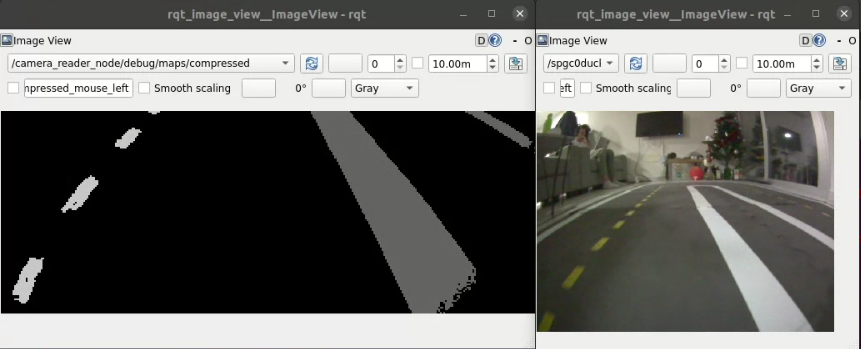
\includegraphics[scale=0.5]{src/Implementation/assets/first_run.png}
    \caption{Output of the first run}\label{fig:first_run}
\end{figure}
During this step, it was discovered that neural network has two problems:
\begin{enumerate}
    \item The whole pipeline of image processing took about 120 milliseconds.
    \item The neural network required a few iterations to speed up.
\end{enumerate}

The first problem was partly solved, but the second remained actual, so it was decided to run a few iterations of the algorithm before sending a signal that 
the Duckiebot is ready to work.

\subsubsection{Torch2trt library}
To solve the first problem described in the previous section it was decided to use the torch2trt library. This library provides an opportunity for easy conversion of  
torch tensors to TensorRT tensors. TensorRT is SDK by Nvidia for high-performance tensor computations. Jetson Nano was developed by Nvidia so there was a hope,
that using this library could increase the speed of computations. This hope was justified. Using torch2trt increased performance twice. However, Installing 
torch2trt wasn't an easy task as it was mentioned in the Docker image subsection. This library couldn't be installed via pip because of the specificity of the hardware, 
building this library from source code was also tricky because the full installation wasn't available due to outdated software in the base Duckietown docker image, 
which couldn't be updated because of backward compatibility problems. 
Luckily partial installation could be performed and this type of installation provided the required speed boost so this half-measure was left.
\subsubsection{Merging neural network and lane-following algorithm}
The merging process was a pretty difficult step. The lane-following algorithm accepts input as a list of segments. 
However, the neural network output is a pixel map of road markup. So it was decided to use the existing algorithm of road markup segmentation but without its main part.
the road markup segmentation part was removed from the existing algorithm. The pipeline is described below:
\begin{enumerate}
    \item Output of neural network is transformed into a multichannel image.
    \item This image is colored into the desired colors: black, white and yellow.
    \item The result is fed into the existing algorithm.
\end{enumerate}  
As a result, the time consumed per image increased by 20 milliseconds, but this approach significantly decreased the time for implementation. 
In addition, because this algorithm was already in use the problem of bugs was also solved. 
\subsubsection{Conclusion}
As a result, the full pipeline for one image takes about 50--70 milliseconds which is a pretty good result. This speed is more than enough for lane following algorithm 
to make decisions on the next action of the Duckiebot.
\subsection{Chapter conclusion}
As it was written in this chapter implementation of the project wasn't an easy task. However, the project was done. There was a lot of research done and a lot of 
code was written, but most of this code was just a utility. The algorithm itself is really small in terms of code volume, however, there was a lot of code behind it, which was
required to write this small amount. 